\documentclass{aip-cp}

\usepackage[numbers]{natbib}
\usepackage{rotating}
\usepackage{graphicx}


%\makeatletter
%\def\@fnsymbol#1{\ensuremath{\ifcase#1\or *\or \dagger\or **\or
%   \ddagger\or \mathsection\or \mathparagraph\or \|\or \dagger\dagger
%   \or \ddagger\ddagger \or\mathsection\mathsection
%   \or \mathparagraph\mathparagraph \or *{*}*\or
%   \dagger{\dagger}\dagger \or\ddagger{\ddagger}\ddagger\or
%   \mathsection{\mathsection}\mathsection
%   \or \mathparagraph{\mathparagraph}\mathparagraph \else\@ctrerr\fi}}
%\makeatother

% Document starts
\begin{document}

% Title portion
\title{OASYS: A Software for Beamline Simulations and Synchrotron Virtual Experiments}

\author[aff1]{Manuel Sanchez del Rio\corref{cor1}} %\noteref{note1,note2}}
%\eaddress[url]{http://www.aip.org}
\author[aff2]{Luca Rebuffi}
%\eaddress{anotherauthor@thisaddress.yyy}

\affil[aff1]{European Synchrotron Radiation Facility, Grenoble (France)}
\affil[aff2]{Elettra Sincrotrone Trieste, Trieste (Italy)}
\corresp[cor1]{Corresponding author: srio@esrf.eu}
%\authornote[note1]{This is an example of first authornote.}
%\authornote[note2]{This is an example of second authornote.}

\maketitle


\begin{abstract}
A modern synchrotron beamline requires an important simulation effort for its design and optimization. OASYS (OrAnge SYnchrotron Suite) is an open-source graphical environment for beamline simulation software designed for that purpose, to perform virtual synchrotron experiments in an efficient, elegant and precise way.

The OASYS environment provides not only an intuitive and very-easy-to-use graphical interface, but also high flexibility and rapidity for interactive simulations. It allows to quickly define and compare multiple configurations in the same workspace to permit optimizing an X-ray instrument. 

OASYS integrates in a synergetic way the most powerful open-source calculation engines available. It interfaces widely used simulation tools for X-ray Optics (e.g. SHADOW for ray tracing, and SRW for wave optics) that are completed with new tools. OASYS provides a mechanism to communicate among the different packages by sending and receiving encapsulated data. The final goal of the OASYS platform is the integration of different packages to completely model synchrotron virtual experiment, retrieving the parameters of the electron beam, calculating the radiation from magnetic structure, then transporting and optimizing the photon beam and eventually including models for interaction with materials to get instrumental functions, study analyzers and detectors and perform ab-initio simulations to support experimental data analysis. 
\end{abstract}


\section{THE PHILOSOPHY OF A VIRTUAL EXPERIMENT: OASYS GOAL}

OASYS (ORange SYnchrotron Suite) is a new graphical environment for modelling X-ray experiments. The goal of the OASYS platform is to make available to the user a collection of different packages to model a synchrotron virtual experiment. From the scientific and algorithmic point of view, OASYS rely on existing well know codes and libraries that are available  thanks to the open-source community. We rely on the open-source mechanism which permits the use of valuable tools developed in synchrotron facilities and made available to the community, and at the same time guarantees due credit to the authors and supporting institutions. Although it is possible to use these codes independently, the users generally get stacked because of installation problems, definition of input parameters, decoding output files and perform data visualization. OASYS integrates in a synergetic way these computational units in a modern and performant graphical environment that facilitates all these tasks, and more important introduces the concept of interoperability or, in other words, the ability of the different units to communicate and exchange information among them. 

OASYS aims to simulating the complete chain of a synchrotron experiment, from the beginning to the end. Thus, the vistual experiment can be decoupled in different steps (see Figure~\ref{figChain0}: 
\begin{enumerate}
 \item Electron beam description and propagation
 \item Photon source: the creation of a photon beam using magnetic structures (insertion devices, bending magnets) placed in the electron beam 
 \item Beamline optics: the description and effect of the individual optical elements or components (slits, mirror, crystals, gratings, etc.)
 \item The interaction with the photon beam with a sample: The detection and analysis of the scattered radiation to get information on the instrumental function (using ideal samples) or on the sample itself via comparison with experimental data. 
\end{enumerate}


\begin{figure}[h]
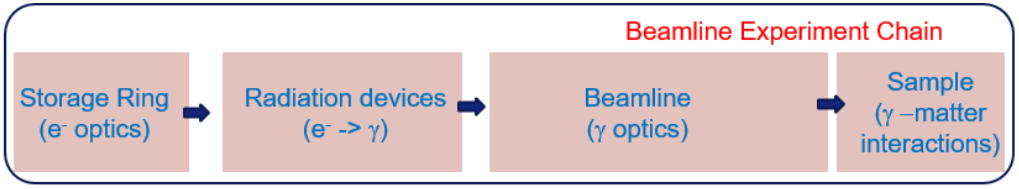
\includegraphics[width=14cm]{FIGURES/chain0.png}
\caption{Schematic workflow of a synchrotron experiment where simulations cover the electron beam, the photon source, the beamline and finally the interaction of the photon beam with the samples.}
\label{figChain0}
\end{figure}

We are conscients of the complexity, dimension and difficulty of such complete simulation in particular if one thinks on the large variety of beamlines and experimental techniques in use. At present, the power of OASYS resides in presenting a modular environment to allow simulations along the complete chain. OASYS now includes powerful tools to make simulations of points 2 (photon sources) and 3 (beamline optics). The ability to be extended to cover the electron beam characteristics and also the interaction with samples is also present and some results are obtained. 

�initio calculate the instrumental function of a synchrotron radiation beamline. This has been successfully tested with an X-ray powder diffraction (XRPD) beamline (Rebuffi and Scardi, 2014) used for line profile analysis, where complete control of the diffracted signal is necessary (Scardi et al., 2010). The synchrotron beam shape, divergence and energy distributions that result from the source characteristics and beamline optics contribute to broaden the diffraction peaks of the recorded diffractograms. The peak width dependence versus the 2θ angle (Caglioti et al., 1958; Sabine, 1987) is usually parameterized by Caglioti's equation (Scardi et al., 1994), where the full width at half-maximum (FWHM) of the instrumental peak profiles represented as pseudo-Voigt curves has the form FWHM(θ) = [W + Vtanθ + Utan2θ]1/2, where W, V and U are Caglioti's parameters and θ is the diffraction angle.




\section{OASYS MECHANISM (CANVAS, WIDGETS AND ADD-ONS). KEY TECHNOLOGIES.}

A main feature of OASYS is to deliver a highly intuitive graphical interface provides high flexibility and rapidity for interactive simulations. OASYS presents an environment for synchrotron radiation virtual experiments. It is presented as a graphical workspace (canvas) that can be populate with applications (widgets) that that communicate among them and are picked up from menus . The applications (widgets)  come from different simulation packages interfaced into OASYS and called add-ons. The different add-ons are optional packages that can be installed or uninstalled from OASYS itself depending on user's convenience. The interesting concept is that the users can add new add-ons depending on their needs. The widgets are connected via ``wires'' that are channels for exchanging information. The kind of information is ``labelled'' in such a way that two widgets can be physically connected if one is capable to emit and the other is able to receive signals that are compatible, i.e., with the same label. In this way the user builds the simulation in a form of workflow containing widgets linked by wires. Every widget has a multiple functionality: it holds the input parameters, triggers a calculation or a data flow and displays results. All these functionality is embedded in a single window that opens by double-clicking the widget. Figure~\ref{figCanvas} presents an example of the canvas and a window from a widget. 
The flowchart concept of the application naturally permits to chain the elements of a virtual experiment. Configurations represented by a single or multiple widgets can be copied, duplicated and changed very quickly to compare multiple configurations. OASYS integrates in a synergetic way the most powerful calculation engines available, that are summarised in the next section. 

\begin{figure}[h]
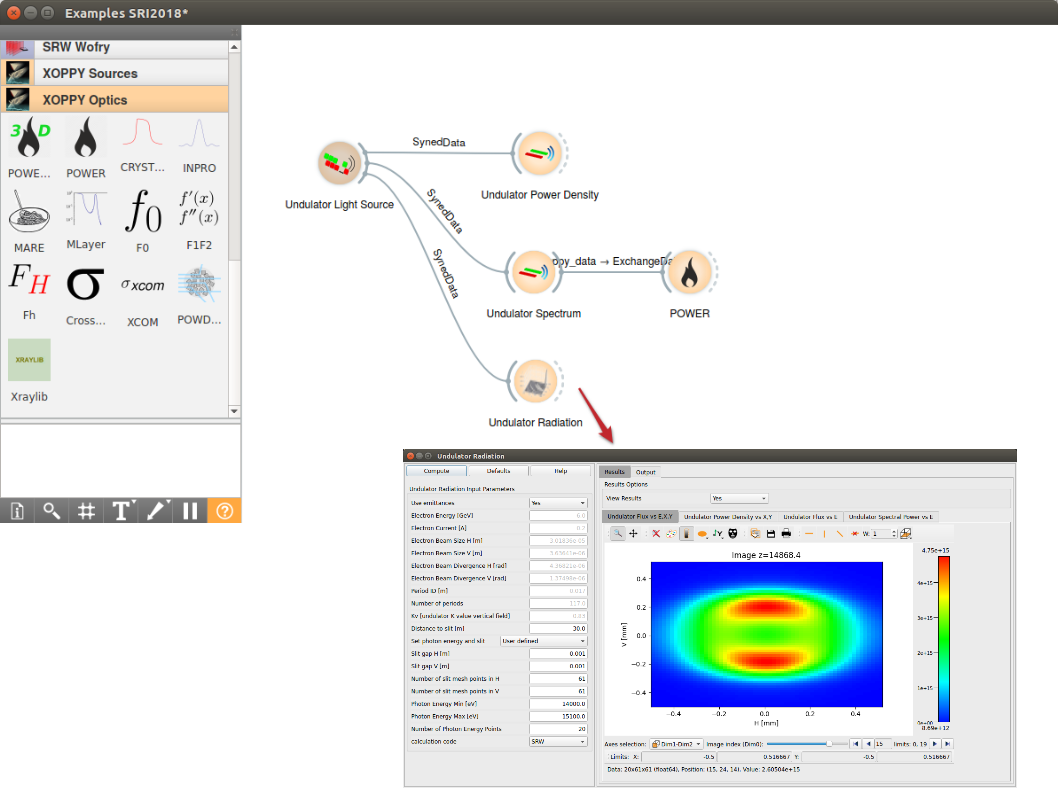
\includegraphics[width=14cm]{FIGURES/canvas.png}
\caption{OASYS application showing on the left area the menu zone containing the installed add-ons, the canvas with some widgets and connections, and a window with the parameters and results of the ``Undulator radiation'' application which computes the flux of an undulators as a function of the horizontal and vertical coordinates and photon energy.}
\label{figCanvas}
\end{figure}


OASYS goal is to become an integration platform where different software packages can communicate by sharing information and results, allowing the user to perform multi-application, complex analyses and simulations easily and safely. To achieve this goal, a careful planning of the technologies to be used and a right selections of the software tools had been done. The boundary conditions imposed are to be open-source, work with open-source tools and be compatible with applications, libraries and packages developed in the academic context. For this reason Python has been selected as main language. It lives a very wide ecosystem with plenty of tools developed by a huge community. 

The OASYS higher level workflow engine that is presented to the user is fully based on the software Orange REFERENCE, developed at the University of Ljubljana (Slovenia). Orange is a Python-based, comprehensive, component-based framework especially designed for data mining and machine learning applications. Orange is designed to simplify the assembly of data analysis workflows and crafting of data mining approaches from a combination of existing components. The Orange suite lumps together several data mining oriented services and applications into a workflow-based interface that provides the interaction with the user and the communication mechanism among the different units. The OASYS higher lever interface derived from the Orange application naked  from its application tools, menus and widgets. OASYS reuses the native Orange main window, canvas, and workflow infrastructure and prompts it to receive the packages we specifically developed for the synchrotron virtual experiments. In addition to Orange workflows, OASYS includes the software elements that are used by several applications (like exchangeable data, loop elements, python scripts, etc.) and installs some common dependencies used by all or several packages (add-ons). Orange widgets are based in {\tt Qt}, thus all user-interface code implements {\tt Qt} functionality. In OASYS all  high level graphics are implemented using the library {\tt silx} REFERENCE developed at ESRF. It contains the necessary applications for displaying 1D, 2D and 3D data and interactive tools for high-level visualization. Coming into more specific scientific applications, most synchrotron simulation codes need to access data for simulating matter-x-ray interactions. The material database for photon-matter cross sections used in OASYS is {\tt xraylib} REFERENCE. {\tt xraylib} provides access to some of the most cited databases of physical data in the field of X-rays. It is used to compute refraction indices, attenuation coefficients, cross sections, crystal structure factors, etc.  OASYS also has {\tt scipy} as a dependency, as it is commonly used for many scientific calculus, fitting, special functions, etc. In particular, the fundamental physical constants should not be directly coded into the applications, as some of them must be updated from time to time following the recommended values the Committee on Data of the International Council for Science (CODATA). OASYS uses the values available in {\tt scipy.constants}.

\section{THE BEAMLINE SIMULATION TOOLS}

The first step before the construction of any X-ray system, such as a synchrotron beamline, is an accurate conceptual design of the optics. The beam should be transported to a given image plane (usually the sample position) and its characteristics should be adapted to the experimental requirements, in terms of flux, energy bandwidth, beam divergence, focal size, time structure, etc.
Today, optical design relies more and more on computer simulation and optimization. 
OASYS integrates different simulation strategies via the implementation of advanced simulation tools for X-ray Optics. We can classify these applications into three groups: i) toolboxes, or applications used for calculating characteristics of sources like spectra or optical elements such as material data, reflectivities, refraction indices, etc. and then simulation of the complete beam using either a ii) ray tracing approach based on geometrical optics valid for mostly incoherent X-ray beams and iii) wavefront propagation useful for beamlines where coherent effects are important and implementing physical optics methods.  

\subsection{The toolboxes (XOPPY, X-ray server, SYNED)}

The ultimate beamline modelling perform a complete simulation including every component of the beamline. For that it is necessary to define every single parameter of the source,  select the appropriated insertion device, define all optical elements including dimensions and positions, etc. In other words, a quite precise beamline description is needed. However, in a first stage of the design, the scientist of engineer would like to check different possibilities of undulators, mirror coatings, monochromator crystal reflection, etc. For that OASYS makes availability different small programs to calculate the individual response of each optical element and characteristics of a particular source, like emitted flux and power. This concept of toolbox has been imported from the code XOP REFERENCE developed in the past which became very popular in many synchrotron facilities. Indeed, all applications of XOP have been ported to python for being integrated into XOPPY, the python version of XOP and available as an OASYS add-on.  

XOPPY lumps together several codes to simulate X-ray sources. They calculate synchrotron radiation sources (spectral emission, angular and spatial distributions, etc.) for undulators, wigglers and bending magnets. For undulators, {\tt Undulator Spectrum} computes the spectral characteristics (emission versus photon energy),  {\tt Undulator Power Density} calculates the emission versus spatial coordinates (x,y) in a screen. In {\tt Undulator Radiation} the radiation is calculated versus three independent variables (x,y, photon energy). The {\tt TC} and {\tt TC-SLIT} calculate tuning curves (emission versus gap variation). These applications interface well known undulator codes ({\tt US, URGENT, SRW, pySRU}). Other applications calculate emission for wigglers ({\tt WIGGLER, WS}), Bending Magnets ({\tt BM}) and X-ray tubes ({\tt TUBE\_W, TUBES}). The {\tt POWER} application can be attached to the source spectrum to calculate the transmission and absorption of some elements (mirrors and filters). These applications are often used to calculate the power deposited and the absorption of the elements, a require input for further finite element analysis to compute thermo-mechanical deformation of the elements. The results of these calculations in terms of surface deformation can be re-injected in OASYS for studying the degradation of the beam, using ray tracing or wave optics simulations. Other applications for reflectivity of optical elements (mirrors, crystals, multilayers) complete the XOPPY package. 

Other add-ons incorporate additional functionality for OASYS. In particular for crystals: the add-on XRAYSERVER implements a front-end of Sergey Stepanov routines available in its widely used web server REFERENCE.  

The availability of different simulation codes in the OASYS environment may need to a redundancy in how the user enters the parameters. For example, the parameters of a mirror (position in the beamline, dimensions curvature, coating, etc.) have to be entered independently in the different codes. 
OASYS defines a uniform and exchangeable description of the real set up (the components of the virtual experiment) tailored to the synchrotron world  flexible enough to allow particularities for different algorithms and physical approaches. This is implemented by creating a framework library that provids the glossary for the definition of light sources and optical components, together with a set of dedicated widgets. This common layer upon OASYS has been called SYNED (SYNchrotron Elements Dictionary), and it is the base for allowing user to create workspaces with several add-ons simulating the same beamline without redundancy, thus separating the description of the real world from details of the calculation algorithms and allowing users to easily benchmark their calculations by using different products for the same simulation. The SYNED description of the beamline components can be stored in {\tt json} files than can be accesible locally (from disk) or remotely (web server). In Figure~\ref{figXoppy} a simple application of SYNED undulator source is used to send the same data to different widgets of XOPPY that calculate different aspects of the source radiation. 

\begin{figure}[hh]
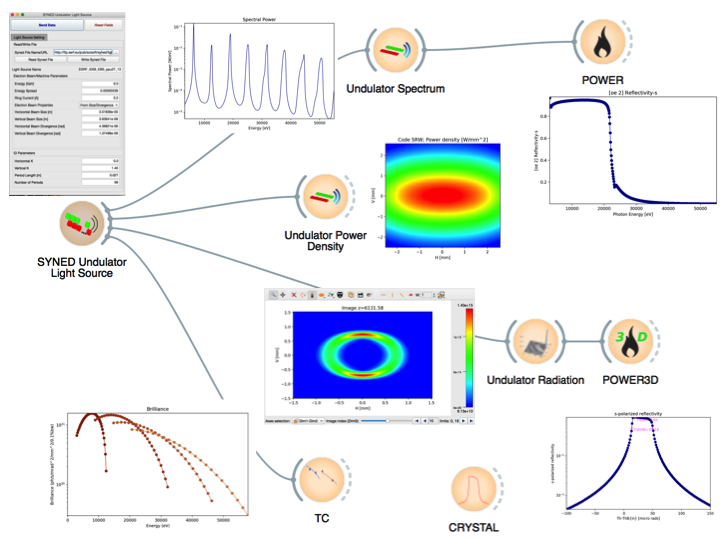
\includegraphics[width=7cm]{FIGURES/xoppy}
\caption{XOPPY.}
\label{figXoppy}
\end{figure}

\subsection{Optics for incoherent optics. Ray-tracing and its environment.}

The ray-tracing technique has been for decades the choice for simulating synchrotron beamlines. Most of the effects that are limiting the performances of X-ray optical elements like source emittance, aberrations, errors in the optical surfaces, etc. can be efficiently modelled by ray tracing. Some particularities of the X-ray optics as compared with visible optics makes impossible that standard commercial optics tools not adequate to synchrotron radiation simulations because, for example, they lack of  a database for refraction indices in the X-ray domain, cannot handle very grazing incident optics and lack of models for perfect crystal diffraction. The code {\tt shadow3} REFERENCE is available in OASYS and via the {\tt ShadowOUI} add-on. This new interface for shadow3 makes a quantum gap in user-friendliness from the old interface in XOP making it more intuitive and incorporating also widgets that permit to define in a very easy way compound optical systems, like CRLs or transfocators. Moreover, ShadowOUI also contains two major new contributions that are introduced here: the Hybrid model and DABAM.

The hybrid method REFERENCE combines ray-tracing and wavefront propagation. One major application of the hybrid method is its ability to assess the effects of figure errors on the performance of focusing mirrors. The hybrid method provides accurate and quick evaluation of the expected mirror performance making it a useful tool for designing diffraction-limited focusing beamlines.

An open-source DAtaBAse for Metrology (DABAM) containing measured profiles of a large collection of X-ray mirrors has been created and interfaced in OASYS. It makes available experimental metrology data (mirror heights and slopes profiles) that can be used with simulation tools for realistic simulations of the effects of optical surface errors in the performances of a synchrotron beamline.


\subsection{Optics for coherent optics. Wavefront propagation.}

In the last years we have witnessed a rapid increase of applications of synchrotron radiation that exploit the beam coherence. Coherence-based techniques such as coherent diffraction imaging (CDI), correlation spectroscopy or more recently ptychography are coping more and more the beamtime  made available at the synchrotron facilities. The availability of a good quality coherent (ideally) or partially-coherent beam is crucial for the success of these experiments. Moreover, working with coherent beams makes more strict the quality exigences of the optical elements: many diffraction inhomogeneities and tripes may appear in the beam structure due to imperfections in the polishing, surface errors, and the use of small numerical aperture optics. It is therefore essential to make available adequate tools for calculating with high accuracy and efficiency the coherence properties of the radiation. 
 
Wave optics methods are computationally more expensive, as usually one has to finely grid the phase space. Hybrid methods permitting to switch from one description to another and vice versa would be ideal. OASYS makes possible the co-existence of software tools that allow treating the same system from two points of view.

The multiple tools dedicated to wave optics and wavefront propagation in OASYS use an integration framework library called WOFRY (Wave Optics FRamework in pYthon). WOFRY has a threefold functionality: i) it provides a generalization (or abstraction) of a software tool for wave optics, combining the component definitions from SYNED with the abstract declaration of wavefronts and propagators, ii) defines a mechanism for interfacing a wave optics code (e.g., SRW, WISE, etc.) in it, a first step for becoming interfaced in OASYS, and iii) provides basic implementations of simple wavefronts (e.g., plane waves, spherical waves, Gaussian sources) and propagators for prototyping optical systems.

For X-ray Optics, OASYS integrates different simulation strategies via the implementation of adequate simulation tools: ray tracing for incoherent optics and and wave optics for fully coherent optics. However, synchrotron radiation is neither incoherent nor coherent, but partially coherent, with a coherent fraction that, for ultimate storage rings, ranges from almost 100\% at low photon energies to a few percent or even less than 1\% for photon energies of tens of keV REFERENCE. Therefore, if one wants to fully describe the coherence properties of the synchrotron beams one can extend the tools to include partial coherence. A first approximated method is the hybrid method mentioned before, that corrects the (incoherent optics) ray tracing results with some coherence effects. This is a method very simple to use in OASYS that can hep in evaluating the impact of coherence in a beamline and assessing on the necessity of using more sophisticated and computationally-expensive partial coherence calculations.  At present, partial coherence calculations are done using two methodologies: i) Monte Carlo sampling of wavefronts from an ensemble of individual electron sampled from the accelerator emittance and functions, and ii) Compute a finite number of well defined wavefronts (coherent modes) that describe in a complete way the statistical properties of the photon beam. The Monte-Carlo has been proposed and it is used in connection with SRW REFERENCE and the second one is implemented in the code COMSYL. Both methodologies will be available in OASYS in a near future.  


\section{OASYS availability, customisation, extensibility}

OASYS is a collaborative freely available and open source project. The code and relative material are available from {\tt https://github.com/oasys-kit}.    OASYS and the available add-ons are continuously developed since 2013.

OASYS provides an interesting platform for developing simulation and data-analysis projects. The infrastructure put in place allows a user with some programming abilities to create his/her own add-ons and integrate them in the OASYS installation. Moreover, users are already creating new add-ons at that extend the functionality current applications (e.g., ShadowOui) with some particular tools. 

At present, the strong point of OASYS is the ability to fully simulate the beamline sources and optics with a complete and variated simulation tools. In the future it will be extended to interactions radiation-samples. An example of this application is an application that simulates the diffracted photon beam created by the interaction of the photon beam generated by shadow3 with a capillary filled by a crystalline material. The simulation takes into account not only the diffraction properties but also the absorption of the photons by the sample material and the sample holder which can be a source of aberrations. The application determine the instrument function of a powder diffraction beamline via an ab-initio  computtion of the Caglioti's parameters.

%\nocite{*}
\bibliography{references}%
\bibliographystyle{aipnum-cp}%



\end{document}
